\section{Experiments}
\label{sec:results}
To demonstrate our superiority over existing methods on segmentation, we first present results on two diverse biomedical image segmentation problems, including synaptic vesicle segmentation and gland segmentation.
To demonstrate the easy extension and generic applicability of our framework, we modified our SCNN to scene text segmentation task.

\subsection{Synaptic vesicle segmentation}
\noindent\textbf{Dataset}
Synaptic vesicle is a good example to evaluate our method, as most of vesicle shape are ellipse.
The images were acquired by . \cxj{by what?}
However synaptic vesicle images are much noisy due to deficient imaging technique.
The plausible vesicles in image are densely arranged and easily confused with other membrane in presynaptic cell, therefore it is hard to obtain clear contour for such dense and small objects.
%The ground truths of dataset are held out by biologists for objective evaluation.
The original dataset is composed of $120$ images with annotations provided by biologists.
The height and width of each image are respectively $1019$ and $1053$, averagely containing $200$ vesicle objects.
Since the average length of a vesicle is about $30$ pixel, we crop a $321\times 321$ region following \cite{Chen2014a} from the original image as the input to network so that each cropped image contain about $25$ objects.
We uniformly crop $25$ patches in each original image with overlap, then the final dataset consists of $3000$ images of $321\times 321$ resolution.

Similar with many existing approaches, we utilize a data augmentation process to reduce overfitting and increase the robustness of our network.
In data augmentation, translation, rotation and image flipping are used to finally produce $8787$ images for training and evaluation.
%\cxj{The final dataset size?}
For better evaluation, a six-fold cross validation is applied in our experiments.
%The first five out of six images are prepared to train our model and the rest of them are used to test its performance.
%\cxj{Six-fold cross validation? or other strategy? }
%
%The validation processing has been repeated several times and the average performance will be reports.


\noindent\textbf{Implementation details.}
We train our network on the open-source deep learning library Caffe~\cite{Jia2014}.
%All the experiments are implemented on a workstation with TitanX GPU cards.
The model of SCNN is well trained by two-step process.
In first stage, we independently train the segmentation branch and shared layers as a general segmentation task.
The parameters of shared layers are initialized from VGG-16 ImageNet pretrained model.
During training phase, the base learning rate was set as $10^{-3}$ and a `step' policy is adopted by decreasing the learning rate by a fact of $10$ every $2000$ iterations.
And mini-batch size was set to $30$ for one iteration with the max iteration number $20000$.
In the second stage, the multi-task FCN as well as two successive joint max pooling layers is jointly fine-tuned based on the model from first stage.
The learning rate of new added layers was set as $10^{-5}$, while the other learning rate was set to $10^{-8}$.
The iteration number of training in second stage is set as $8000$.
Especially, joint max pooling requires multiple iterations $L$ to optimize as many shape predictions in boundary area as possible.
And the optimal $L$ together with pooling size $k_s$ will be jointly explored in subsequent experiment.
The balancing weight $\alpha$ in Eq.~\ref{EqLoss} was determined by fixing $\alpha L=20$, of which the value $20$ is calculated according to the ratio of positive and negative labels of the whole dataset.
For fusing step, the important thresholds $\tau_1$ and $\tau_2$ are also explored in latter experiment, which determine the degree of prior shape constraint in final segmentation mask.

\noindent\textbf{Evaluation setup.}
%
The evaluation criteria in our experiments includes an score $F_1$ to evaluate performance of object detection and a pixel intersection-overunion (IOU) averaged across different classes to evaluate the segmentation accuracy .
%The $F_1$ score considers the performance of object detection, while IOU consider the segmentation performance, respectively.

For detection, the $F_1$ score is defined as:
%
\begin{eqnarray}\label{EqF1}
\begin{aligned}
F1 = \frac{2PR}{P+R}
\end{aligned}
\end{eqnarray}
where $P$ is the detection precision and $R$ is the detection recall.
Especially, a true positive detection is the segmented object that intersects with at least $50\%$ with the ground truth, otherwise it is regarded as a false positive.
If a ground truth object has no corresponding segmented object that intersects more than $50\%$, it is regarded as a false negative.

The IOU metric for segmentation accuracy is defined as:
%
\begin{eqnarray}\label{EqIou}
\begin{aligned}
IOU = \frac{1}{N_s}\sum_{i=1}^{N_s}\frac{|G_i\bigcap S_i|}{|G_i\bigcup S_i|}
\end{aligned}
\end{eqnarray}
%
where $N_s$ denotes the number of pixel label.
$G_i$ denotes the pixel set with $i$-th label in ground truth .
$S_i$ denotes the pixel set with $i$-th class in segmented result.
In our object segmentation task, there are two kind of labels: object or background, therefore $N_s$ is set to $2$.
\begin{figure*}
    \begin{center}
        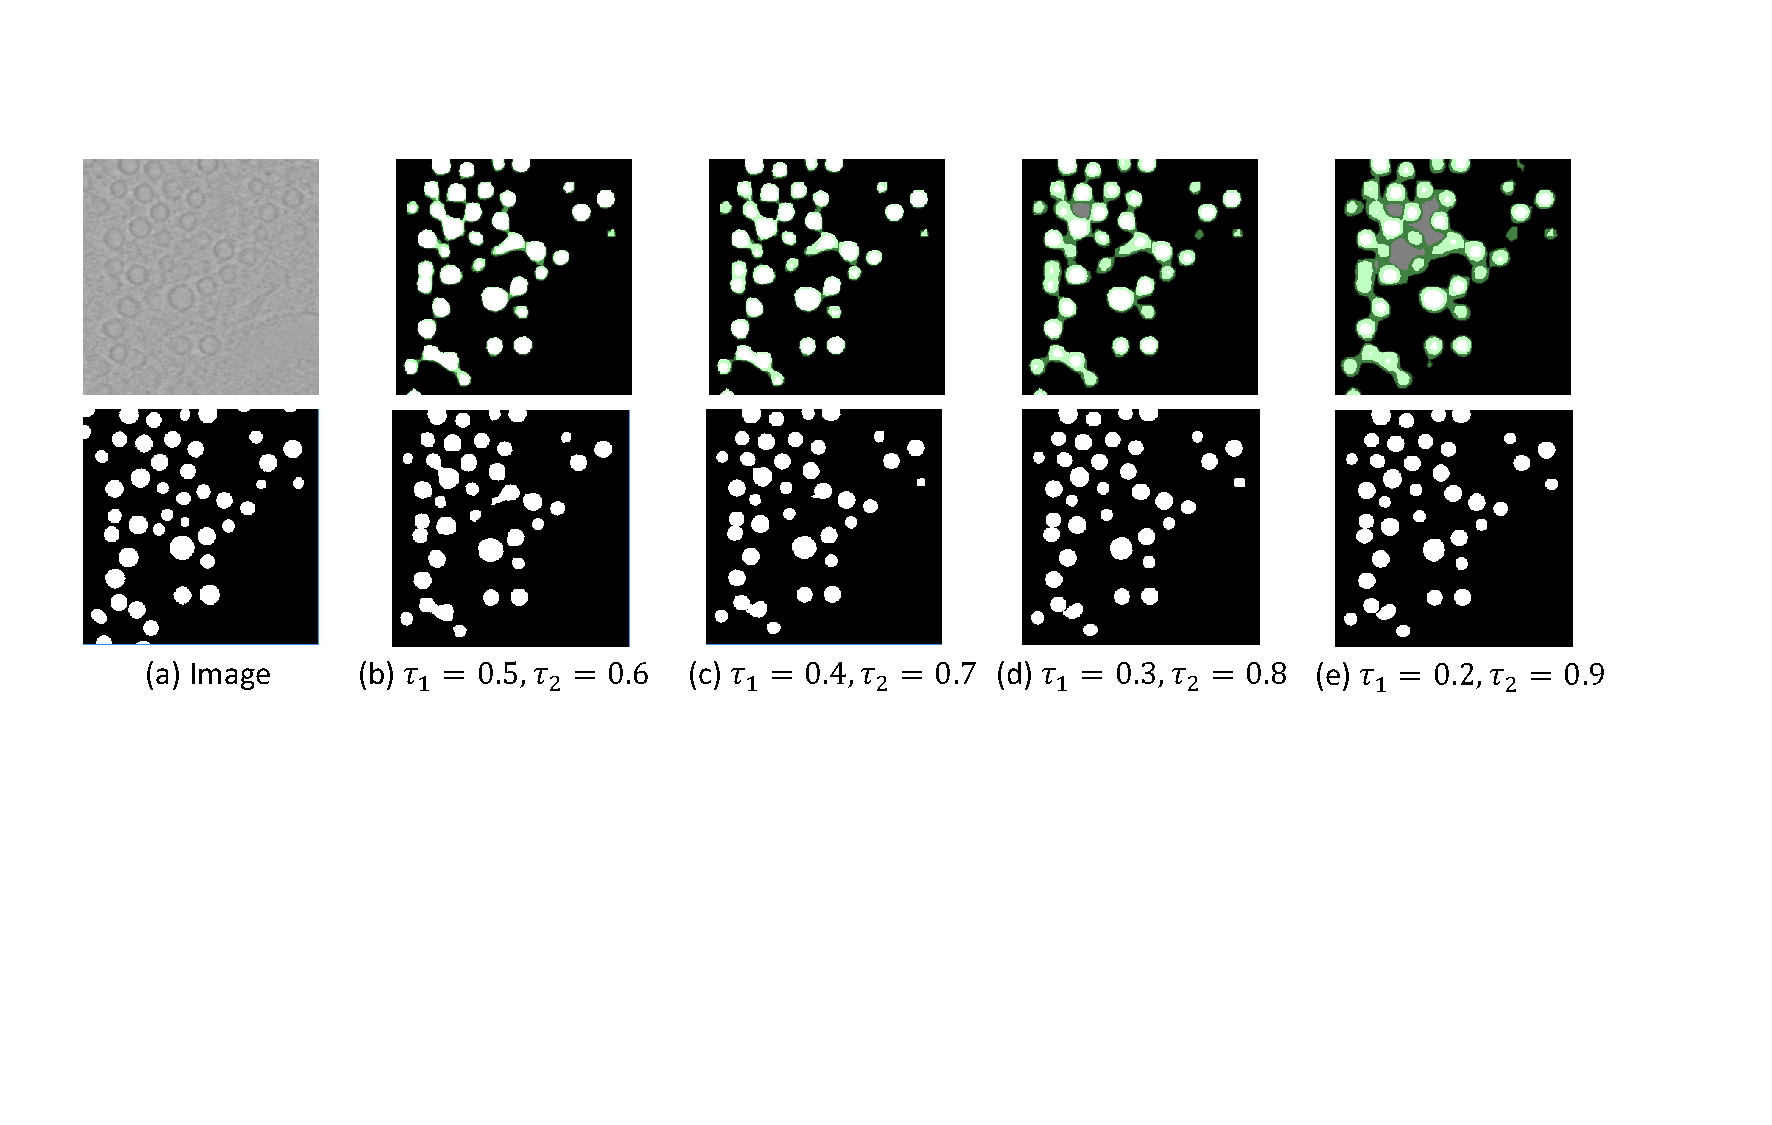
\includegraphics[width=7in]{figures/FigCon.pdf}
    \end{center}
    \caption{Effect of varying fusion thresholds $\tau_1$ and $\tau_2$ with $\varepsilon=9$. First row contains the input image and raw segmentations from bojectness score, where the pixels of objectness score between $[\tau_1,\tau_2]$ has been highlighted. Second row contains the ground truth and optimized segmentations of varying $[\tau_1,\tau_2]$. It shows that a large interval of $[\tau_1,\tau_2]$ means the stronger shape constraints to the segmented objects.}
    \label{FigCon}
\end{figure*}


\begin{figure*}
    \begin{center}
        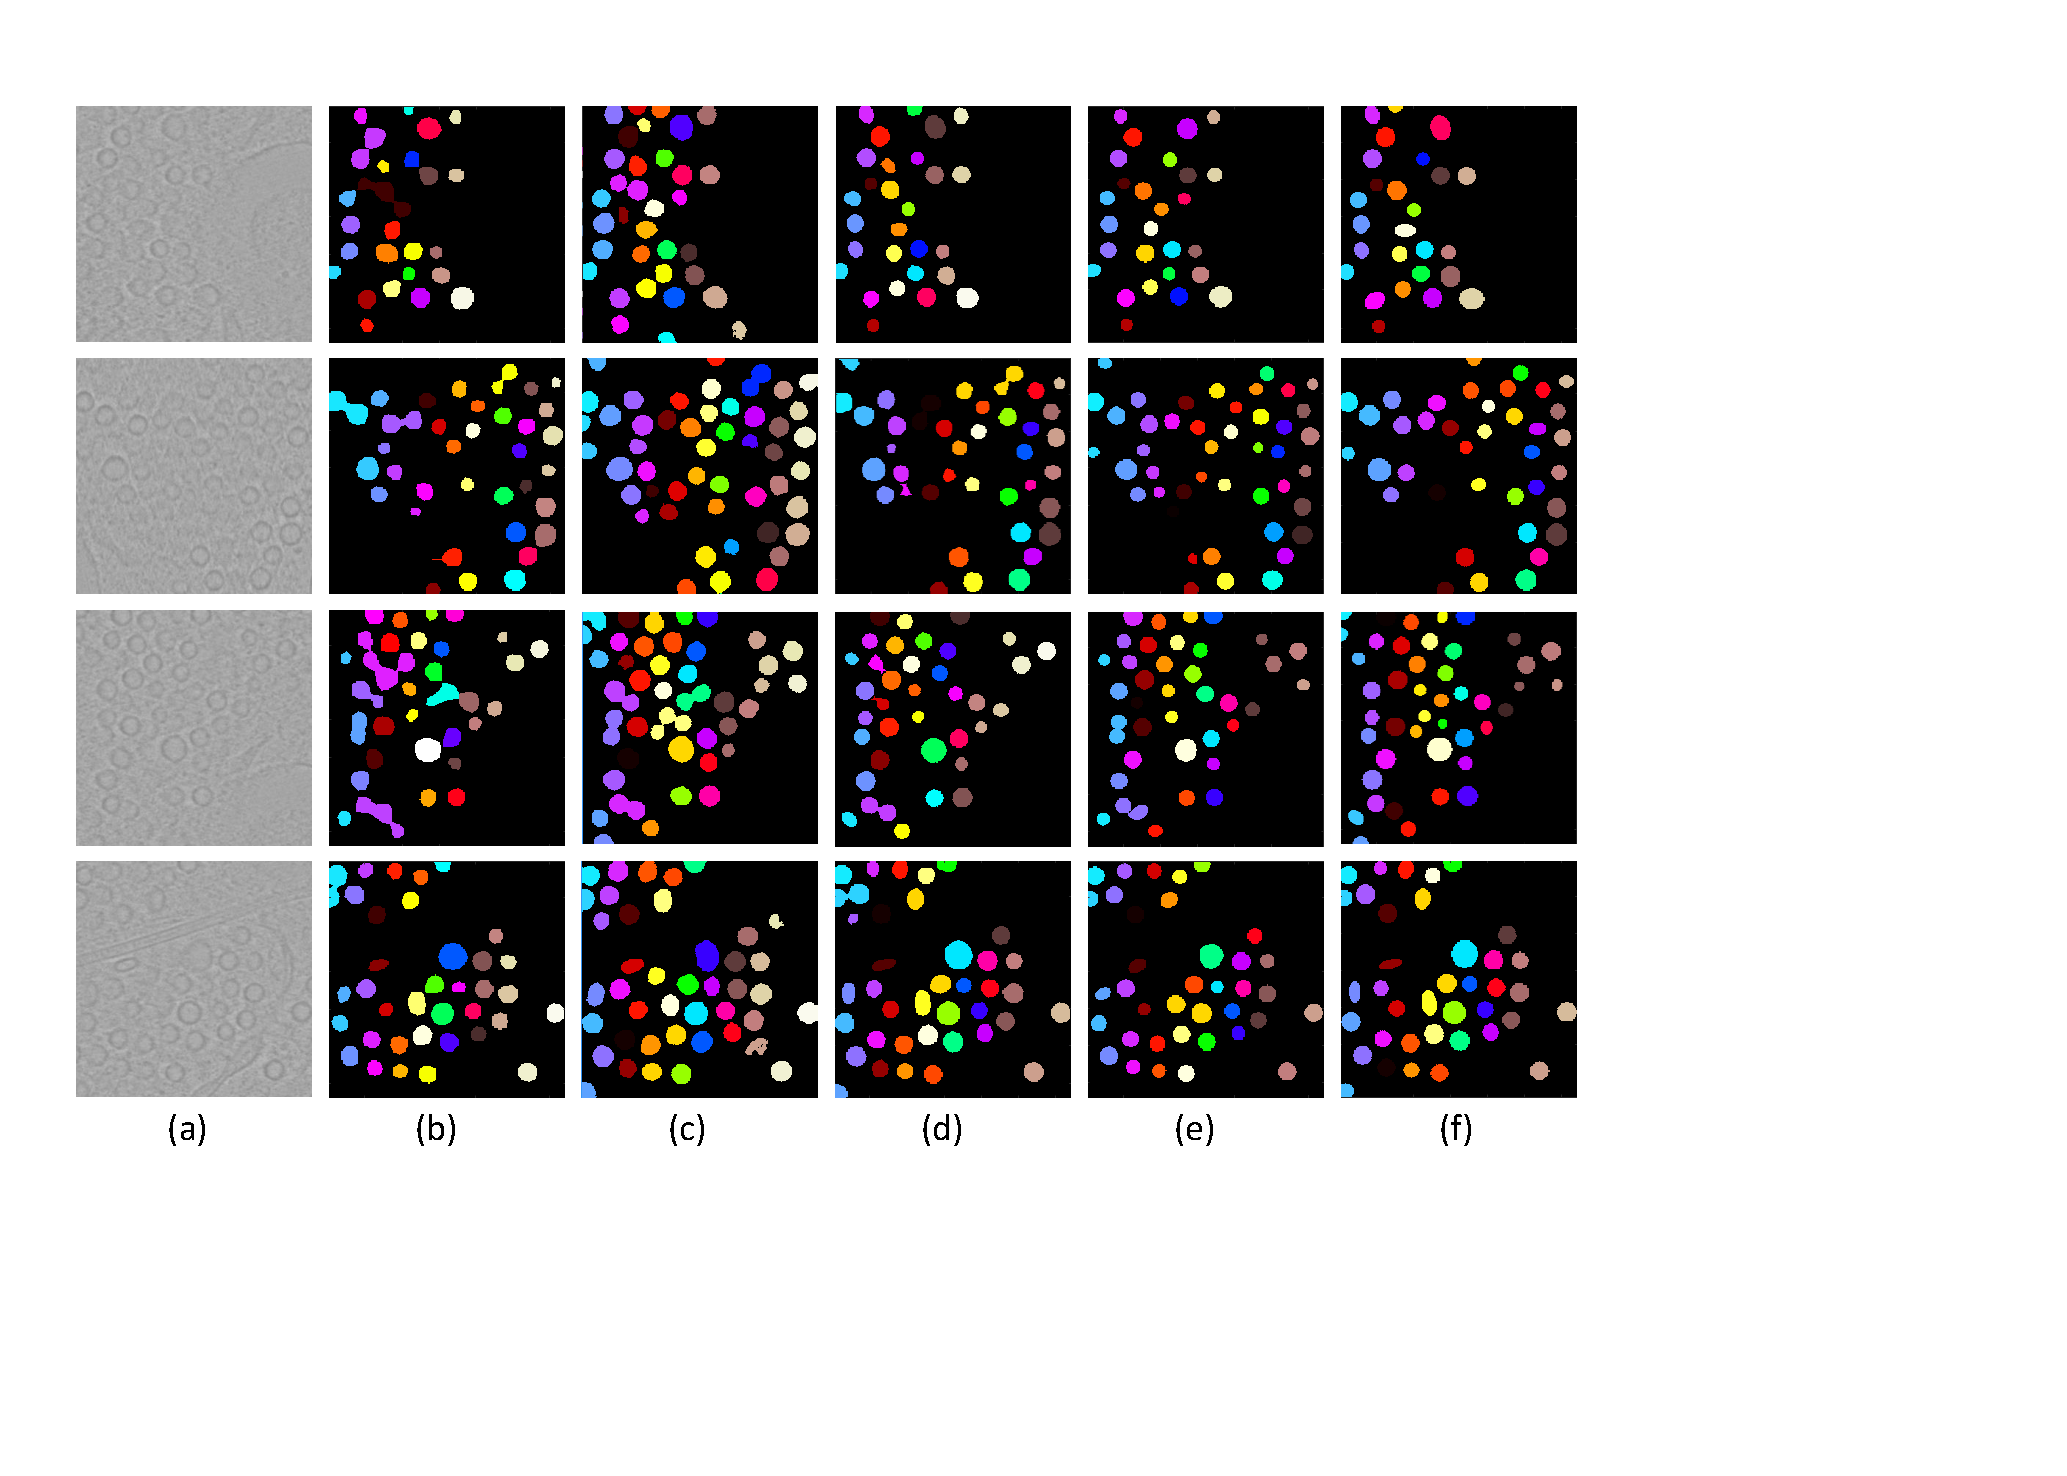
\includegraphics[width=7in]{figures/FigVesicle.pdf}
    \end{center}
    \caption{Some segmentation results of synaptic vesicle: (a) the input image; (b)-(f) the segmentation respectively from deeplab, u-net, DCAN, $SCNN^{-1}$ and SCNN; (g) the ground truth.}
    \label{FigVesicle}
\end{figure*}

\noindent\textbf{Exploring the effect of $\{L, k_s, \tau_1, \tau_2\}$ to final segmentation.}
In this experiment, the effect of different $L$, $k_s$, $\tau_1$, $\tau_2$ for segmentation performance is jointly investigated and the optimal solution will be searched.
In order to reduce the hyper-parameters, we use $\varepsilon=\frac{(L-1)k_s}{2}$ to simultaneously represent $L$ and $k_s$ , because the influence of both $L$ and $k_s$ to the whole network is the reception field of joint max pooling layers.
Therefore, we first fix $\tau_2=0.7$ and vary $\tau_1$ to observe its effect of different $\varepsilon$ as shown in Figure~\ref{FigVar} (a).
Then, $\tau_1$ is fixed in turn and $\tau_2$, $\varepsilon$ are varied in Figure~\ref{FigVar}  (b).
Observed from Figure~\ref{FigVar} , it is properly to employ $\varepsilon=9$ for vesicle segmentation to obtain most of the gains for different $\tau1$ and $\tau2$.
In practice, we set $k_s=9$ and $L=3$ to satisfy the condition of $\varepsilon=9$, which reaches a balance between speed and effect.
For $\tau_1$ in Figure~ (a), we fine that $\tau_1=0.2$ is the best lower threshold when $\varepsilon=9$.
And fixing $\tau_1=0.2$, $0.9$ is found to be the optimal value of $\tau_2$ according to Figure~\ref{FigVar} (b).
Finally, we use a large interval of $[0.2, 0.9]$ as the thresholds in Eq.~\ref{fusion} to impose a strong shape restriction, because the shape of most synaptical vesicles are regular ellipse.
Especially, $\varepsilon=0$ means no joint max pooling applying to network.
Besides finding the optimal values of $\tau_1$ and $\tau_2$, it can be found that the segmentation accuracy is coarsely positive correlation to $\varepsilon$ in  Figure~\ref{FigVar} .
This demonstrate the effectiveness of our JMP in improving the accuracy of predicted shape parameters in boundary area with increasing $\varepsilon$.
And an interesting observation is that the effect of varying $\tau_2$ to final segmentation is not as obvious as varying $\tau_1$.
This is because that most misclassified pixels comes from the touching area, whose objectness scores $P_i$ are lower and approximate to $0.5$ shown in Figure~\ref{FigVesicle}.
Furthermore, we presents some examples of different $[\tau_1,\tau_2]$ in Figure~\ref{FigCon} to illustrate how these thresholds control the degree of prior shape constraint to segmented objects.

\begin{figure}
    \begin{center}
        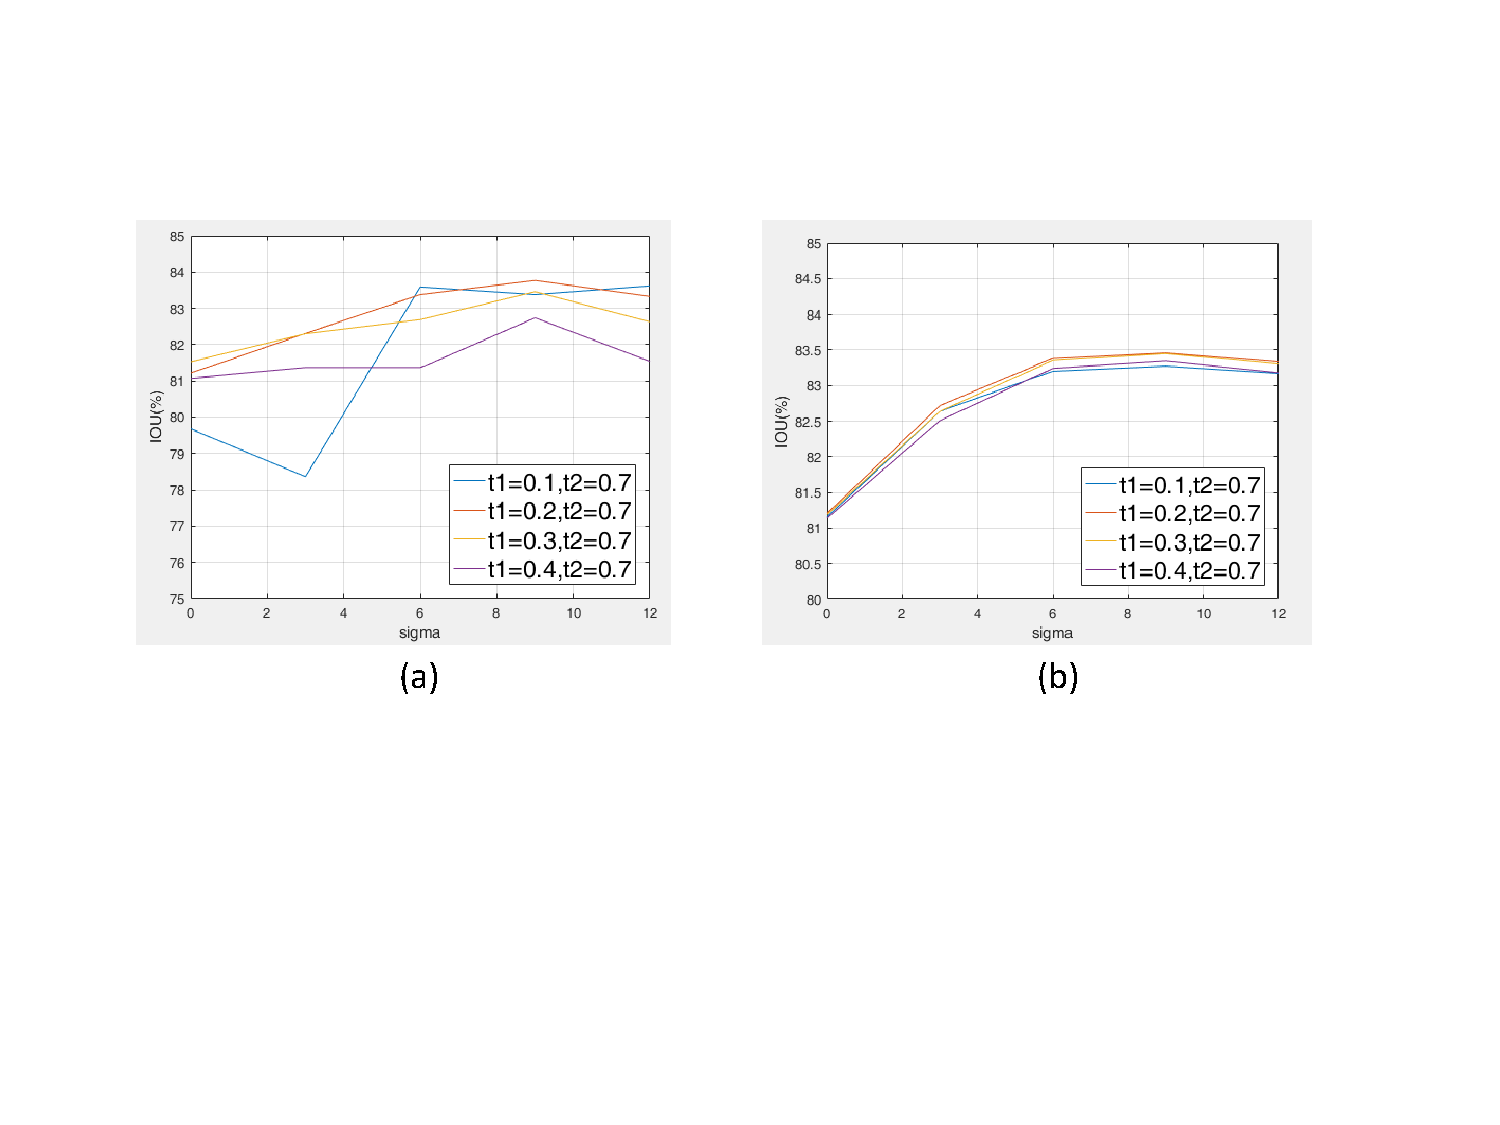
\includegraphics[width=3.5in]{figures/FigVar.pdf}
   %\includegraphics[width=0.8\linewidth]{egfigure.eps}
    \end{center}
    \caption{Effect of varying $\varepsilon$ for vesicle segmentation: (a)Fix $\tau_2$ and vary both $\tau_1$ and $\varepsilon$. (b) Fix $\tau_1$ and vary both $\tau_2$ and $\varepsilon$.}
    \label{FigVar}
\end{figure}

\noindent\textbf{Qualitative evaluation on synaptic vesicle segmentation}
Figure \ref{FigVesicle} shows some segmentation results of testing data.
In order to verify the effectiveness of parameterized shape information, we compared our method with DeepLab \cite{Chen2014a}, u-net~\cite{Ronneberger2015} without any complementary information and DCAN~\cite{Chen2016a} with contour map as auxiliary.
Furthermore, we also present the results of $SCNN^{-}$ that remove the joint max pooling layers from SCNN to prove its effectiveness.
The fusing thresholds follow the optimal setting in previous experiment.

From Figure \ref{FigVesicle}, we can see that without other complementary information, there exists many touching objects that cannot be separated by DeepLab (Figure~\ref{FigVesicle} (b)).
This is because that the contours of many synaptic vesicles are very fuzzy and incomplete due to deficient imaging technique as shown in Figure~\ref{FigVesicle} (a).
And the dense synaptic vesicles around presynaptic membrane increase the difficulty to separate them into individual ones.
Also without auxiliary, u-net (Figure~\ref{FigVesicle} (c)) is superior than DeepLab in terms of touching problem due to the U-shape network that supplements many context information to higher resolutions layers.
However, the raw context information added to higher layers brings more false detection into the segmentation, because of the coarse raw image quality.
Although DCAN is capable to separate touching synaptic vesicles apart in Figure~\ref{FigVesicle} (e), it also produced additional false detections by cutting the touching vesicles with respective contours.
When the connection region between two touching vesicles are wide and large, cutting the touching regions by respective contours will generate an additional positive region besides two separated vesicle objects.
Differen from the above methods, our SCNN uses the shape parameters of objects as complementary information to separate the touching object clearly without residual regions.
As the results in Figure~\ref{FigVesicle} (f), all the touching objects have been well separated and their shape are more smooth and regular.
And the comparing result of Figure~\ref{FigVesicle} (e) prove again the effectiveness of joint max pooling by improving the accuracy of shape parameters.

\noindent\textbf{Quantitative evaluation.}
To quantitatively evaluate our method, we compare the object detection rate $F_1$ and the segmentation accuracy IOU of our SCNN with the state of the art segmentation methods based on Deeplab~\cite{Chen2014a}, u-net~\cite{Ronneberger2015} and DCAN~\cite{Chen2016b}, which are commonly used in biomedical image process.
Their results on our synaptic vesicle dataset are shown in Table~\ref{tab:vesicle}.
And we further implement $SCNN^{-}$ that is the clipped version of SCNN without joint max pooling.
Their results are also presented in Table~\ref{tab:vesicle} to prove effectiveness of our joint max pooling.

From F1 score obtained in Table~\ref{tab:vesicle}, the performance of SCNN surpassed the other methods.
The common low F1 scores are caused by difficulty in detecting dense synaptical vesicles in such noise background.
Especially, we observed that the performance of u-net obtained about $3\%$ improvement over DeepLab, both of which did not use any auxiliary supervised information.
This arises from the fact that U-shape applied in u-net is effective to alleviate touching problem, which confirmed that missing of context information is a significant factor of touching problem in biomedical segmentation.
Furthermore, we noticed that there is not much improvement of F1 score obtained by DCAN compared to u-net and DeepLab.
This is because that many false detection region between two objects, separated by predicted contours, increase the false positive scores in Eq.~\ref{EqF1}, shown in Figure~\ref{FigVesicle} (d).
And $SCNN_{-}$ gives a lower F1 score compared to SCNN, because of some touching cases caused by inaccurate auxiliary information predicted in boundary area.

From IOU metrics in Table~\ref{tab:vesicle}, our SCNN gives the best performance again among various methods.
It should be noted that although the other methods also obtain a good IOU score, their contours are more coarse and irregular as shown in Figure~\ref{FigVesicle}, which increase the difficulty of subsequent processing such as reconstruction of 3D structure.
And the segmented vesicle by our SCNN are more clear and regular.
Moreover, the results demonstrate that our joint max pooling operation can effectively improve the accuracy of predicted shape parameters, which leads to a better performance on objects shape.
Both qualitative and quantitative evaluations present the superiority of our SCNN in segmenting densely arranged objects with regular and small objects by incorporating the prior shape knowledge into network.

\begin{table}
\begin{center}
\begin{tabular}{lcc}
\hline
Method & F1($\%$) & IOU($\%$) \\
\hline
DeepLab & 66.75 & 80.95 \\
U-net & 69.99 & 77.56 \\
DCAN & 70.94 & 80.61 \\
$SCNN^{-}$ & 74.52 & 81.04 \\
SCNN & $\mathbf{75.68}$ & $\mathbf{83.34}$\\
\hline
\end{tabular}
\end{center}
\caption{The detection and segmentation results of different methods in our synaptic vesicle dataset.}
\label{tab:vesicle}
\end{table}

\subsection{Gland segmentation}
\textbf{Dataset}
In this section we present SCNN for segmenting benign and malignant gland.
We consider the public dataset of \emph{Gland Segmentation Challenge Contest} in MICCAI2015~\cite{Sirinukunwattana2015a}.
%
The training dataset is composed of 85 images, consisting of 37 benign and 48 malignant, with ground truth annotations provided by expert pathologists.
Especially, there is a huge variation of glandular morphology in malignant case, which can prove the generalization of our SCNN to irregular objects.
The same data augmentation in vesicle segmentation is implemented for a better performance.

\textbf{Implementation details}
Because there exists many irregular objects in gland images that we desire to remain more contour information obtained by object prediction, the contour modification by parameterized contour information should be relatively weaker than segmenting vesicles.
By experimental verification, we find that $\tau_2=0.7$ and $\tau_1=0.4 $ produce a better results.
\cxj{So show comparison of results using different parameters.}
%
And we still use the standard elliptic parameter as the prior shape constraint for gland, as most benign glands and few malignant glands' shape are approximate ellipses.
The other implementation settings and evaluation metrics follow the vesicle segmentation.

\textbf{Qualitative evaluation on gland segmentation}
Follow previous qualitative evaluation, we presented the results of u-net and the state of art method DCAN in gland segmentation with our SCNN in Figure~\ref{fig:com-gland}.
The first two columns are the examples of benign gland images, and the rest two columns are the examples of malignant images.
From the results, we can observed that both SCAN and SCNN can well solve the touching problem in benign and malignant cases.
However for benign case, the contours of glands obtained by SCNN are more smooth than that of DCAN.
And for malignant case, since SCNN only modify the segmentation predictions on the object border, there is no obvious deterioration compared to DCAN.

\begin{figure}
	\centering
	\vspace{0.4in}
	\caption{\cxj{Add comparison of gland segmentation with U-net and DCAN.}}
	\label{fig:com-gland}
\end{figure}

\textbf{Quantitative evaluation}
Table \ref{} shows the F1 score and IOU metric over the $Gland$ $Segmentation$ $Challenge$ $Contest$ by several commonly used biomedical segmentation methods.

\begin{table}
	\centering
	\caption{Performance comparison on gland segmentation.}
	\begin{tabular}{c|cc}
		\hline
		Method & F1 & IOU \\
		\hline
		DeepLab & 0 & 0 \\
		U-Net & 0 & 0 \\
		DCAN & 0 & 0 \\
		SCNN-v1 & 0 & 0 \\
		SCNN-v2 & 0 & 0 \\
		\hline
	\end{tabular}
\end{table}


\subsection{Scene text detection}
We further extended SCNN to scene text detection task, which
